\documentclass{beamer}
\usetheme{Singapore}
\usepackage[english]{babel}
\setbeamertemplate{navigation symbols}{}
\setbeamertemplate{frametitle}[default][center]
\setbeamertemplate{bibliography item}{\insertbiblabel}
\usefonttheme[onlymath]{serif}

\usepackage{graphicx}
\graphicspath{ {./Images/} }
\usepackage{amsmath}
\usepackage{wrapfig}

\title{Research Presentation}
\subtitle{COMP230}
\author{1702208}

\begin{document}

\begin{frame}
	\maketitle
\end{frame}

\begin{frame}{Background}
	Nowadays video games have become a very common way of spending time among adolescents. Playing games have both negative and positive effects. Positive effects are usually stress reduction\cite{russoniello2009effectiveness}, relaxation\cite{wack2009relationships}, emotional disturbances in children\cite{jones2014gaming}\cite{hull2009computer} and a lot more. But there are still some negative consequences. Besides the most common - addiction - there are aggression, antisocial behaviour and violence, that usually depends on the game itself.
\end{frame}

\begin{frame}{Massive Multiplayer Online Role-Playing Games}
	There are a lot of studies about MMORPGs, where the most common subject is World of Warcraft. It's a unique game to study for game ethics as it can bring both positive and negative results. The game is either a way to relax and reduce stress - usually for casual players - or ``risky addiction-like experiences"\cite{snodgrass2011magical}. 
\end{frame}

\begin{frame}{Violence}
	Violence in games usually depends on the game itself and how players will see it. But there are definitely games that only focus on violence and were restricted or censored in some countries. One of which is Hatred. Nevertheless there are still games that show violence and aren't restricted by any manner.
\end{frame}

\begin{frame}{Social or Anti-social?}
	\frametitle{}
	\begin{columns}
		\column{0.5\textwidth}
		People that spend most their time playing games are usually considered as antisocial people. But playing different types of games require different contribution with other players, such are shown in figure \ref{fig:gtypes}. Therefore, it's hard to say for sure, as it includes many factors.
		\column{0.5\textwidth}
		\frametitle{}
		\begin{figure}
			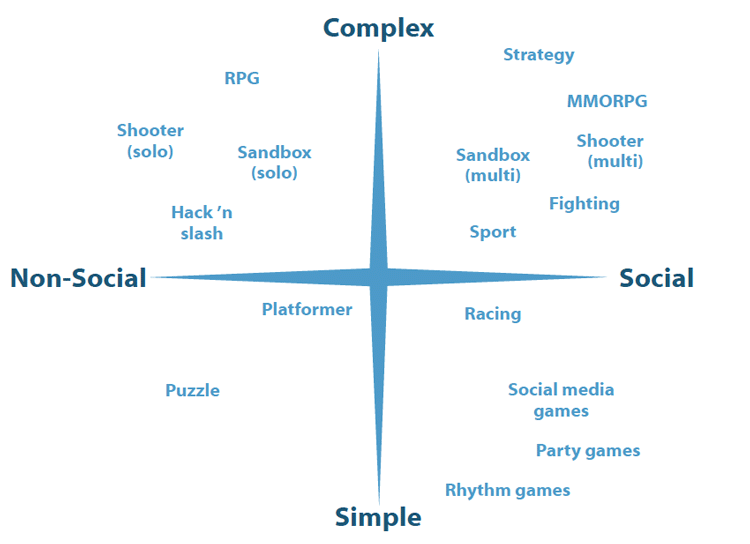
\includegraphics[width=\linewidth]{all-video-game-genres-2}
			\caption{Game Types.}
			\label{fig:gtypes}
		\end{figure}
	\end{columns}
\end{frame}

\begin{frame}{Research Question}
	What mental consequences video games bring? \vspace{5mm}
	\begin{itemize}
		\item Is it developers intention to make games addictive?
		\item Why gamers play violent games and does it influence them?
		\item Does preferable game type make players sociable or dissociable respectively?
	\end{itemize}
\end{frame}

\begin{frame}[allowframebreaks]{References}
	\bibliographystyle{ieeetran}
	\bibliography{references}
\end{frame}
\end{document}